
\textbf{Pour cette première partie, aucune justification n'est demandée et une seule réponse est possible par question. Pour chaque question, reportez son numéro sur votre copie et indiquez votre réponse.}

\subsubsection*{Question 1}
Jean consacre 25\% de sa journée de dimanche à faire ses devoirs. \\
80\% du temps consacré aux devoirs est consacré à faire un exposé.

Le pourcentage du temps consacré à l'exposé par rapport à la journée de dimanche est égal à :

\textbf{a.} 80\% - 25\% \hfill \textbf{b.} $\dfrac{1}{4} \times 80\%$

\textbf{c.} $0,08 \times 25\%$ \hfill \textbf{d.} Cela dépend de la durée de la journée de dimanche.

\subsubsection*{Question 2}
Un prix diminue de 50\%. Pour retrouver le prix initial, il faut une augmentation de :

\textbf{a.} 50\% \hfill \textbf{b.} 100\% \hfill \textbf{c.} 150\% \hfill \textbf{d.} 200\%

\subsubsection*{Question 3}
Le prix d'une tablette a baissé : il est passé de 250 euros à 200 euros. \\
Cela signifie que ce prix a été multiplié par :

\textbf{a.} 1,25 \hfill \textbf{b.} 0,75 \hfill \textbf{c.} 0,8 \hfill \textbf{d.} $-0,8$

\subsubsection*{Question 4}
La seule égalité vraie est :

\textbf{a.} $40 \times \dfrac{1}{40^3} = 40^2$ \hfill \textbf{b.} $(2^{-4})^3 = 2^{-1}$ \hfill \textbf{c.} $\dfrac{10^{-5}}{10^8} = 10^{-13}$ \hfill \textbf{d.} $5^{-6} \times 11^{-6} = 55^{-12}$

\subsubsection*{Question 5}
L'épaisseur d'une feuille de papier est égale à $70 \times 10^{-3}$ mm. \\
L'épaisseur d'une pile de 2\,000 feuilles est égale à :

\textbf{a.} 140 cm \hfill \textbf{b.} 14 mm \hfill \textbf{c.} 14 cm \hfill \textbf{d.} 72 cm

\subsubsection*{Question 6}
Voici quatre planètes et leur masse.

\begin{center}
\begin{tabular}{|c|c|}
\hline
Terre & $5\,973 \times 10^{21}$ kg \\
\hline
Mercure & $33,02 \times 10^{22}$ kg \\
\hline
Vénus & $48\,685 \times 10^{20}$ kg \\
\hline
Mars & $6,4185 \times 10^{23}$ kg \\
\hline
\end{tabular}
\end{center}

La planète dont la masse est la plus importante est :

\textbf{a.} Terre \hfill \textbf{b.} Mercure \hfill \textbf{c.} Vénus \hfill \textbf{d.} Mars

\subsubsection*{Question 7}
On additionne un nombre réel $x$, avec son triple et son carré. Le résultat est égal à :

\textbf{a.} $(x + 3x)^2$ \hfill \textbf{b.} $x + (3x)^2$ \hfill \textbf{c.} $1 + 3x^2$ \hfill \textbf{d.} $4x + x^2$

\bigskip

\begin{minipage}[t]{0.65\textwidth}
\subsubsection*{Question 8}
Dans la figure ci-contre, les courbes $C$ et $C'$ représentent respectivement les fonctions $f$ et $g$. \\
L'ensemble des solutions de l'inéquation $f(x) \leq g(x)$ est :

\textbf{a.} $[-2~;~-1]$ \hfill \textbf{b.} $[1~;~2]$ \\
\textbf{c.} $[-2~;~-1] \cup [1~;~2]$ \hfill \textbf{d.} $[-2~;~-1] \cap [1~;~2]$
\end{minipage}
\hfill
\begin{minipage}[t]{0.3\textwidth}
\vspace{0pt}
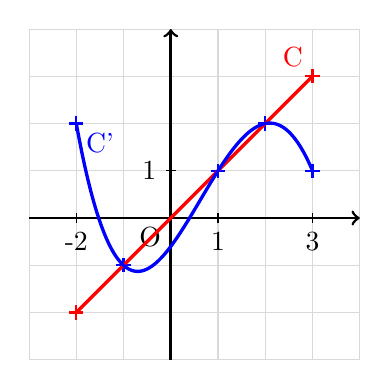
\begin{tikzpicture}[scale=0.6]
\draw[gray!30] (-3,-3) grid (4,4);
\draw[->, line width=1pt] (-3,0) -- (4,0);
\draw[->, line width=1pt] (0,-3) -- (0,4);
\foreach \x in {-2,1,3} {
\draw (\x,0.1) -- (\x,-0.1) node[below] {\x};}
\foreach \y in {1} {
\draw (0.1,\y) -- (-0.1,\y) node[left] {\y};}
\node[below left] at (0,0) {O};
\foreach \x/\y in {-1/-1, -2/2, 1/1, 2/2, 3/1} {
\draw[blue, thick] (\x,\y) ++(-0.15,0) -- ++(0.3,0);
\draw[blue, thick] (\x,\y) ++(0,-0.15) -- ++(0,0.3);}
\foreach \x/\y in {-2/-2, 3/3} {
\draw[red, thick] (\x,\y) ++(-0.15,0) -- ++(0.3,0);
\draw[red, thick] (\x,\y) ++(0,-0.15) -- ++(0,0.3);}
\draw[red, very thick] (-2,-2) -- (3,3);
\node[red, above left] at (3,3) {C};
\node[blue, below right] at (-2,2) {C'};
\draw[blue, very thick, smooth, samples=200, domain=-2:3]
plot (\x, {((\x)^4)/60 - (1/3)*(\x)^3 + (7/12)*(\x)^2 + (4/3)*(\x) - 0.6});
\end{tikzpicture}
\end{minipage}

\bigskip

\begin{minipage}[t]{0.6\textwidth}
\subsubsection*{Question 9}
On donne ci-contre la courbe représentative $C$ d'une fonction $f$ définie sur l'intervalle $[-3~;~2]$. On s'intéresse à l'équation $f(x) = 0$. \\
Une seule de ces propositions est exacte :

\textbf{a.} L'équation $f(x) = 0$ n'admet aucune solution. \\
\textbf{b.} L'équation $f(x) = 0$ admet exactement une solution. \\
\textbf{c.} L'équation $f(x) = 0$ admet exactement deux solutions, et ces solutions sont négatives. \\
\textbf{d.} L'équation $f(x) = 0$ admet exactement deux solutions, et ces solutions sont de signes contraires.
\end{minipage}
\hfill
\begin{minipage}[t]{0.35\textwidth}
\vspace{0pt}
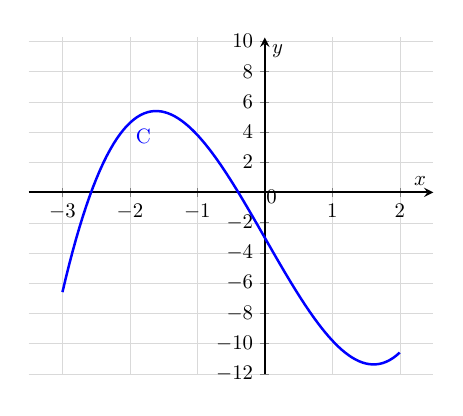
\begin{tikzpicture}[scale=0.75]
\begin{axis}[
xmin=-3.5, xmax=2.5,
ymin=-12, ymax=10.25,
samples=100,
axis lines=middle,
xlabel=\(x\),
ylabel=\(y\),
restrict y to domain=-12:10.25,
axis line style={line width=1pt},
ytick distance=2,
grid=both,
grid style={line width=.1pt, draw=gray!30},
]
\addplot[blue, very thick, domain=-3:2] {x^3 - 7.8*x - 3};
\node at (axis cs:0.1,-0.3) {0};
\node[blue] at (axis cs:-1.8,3.7) {C};
\end{axis}
\end{tikzpicture}
\end{minipage}

\subsubsection*{Question 10}
On considère une fonction $f$ définie sur $\mathbb{R}$ dont le tableau de signes est donné ci-dessous.

\begin{center}
\begin{tabular}{|c|ccccc|}
\hline
$x$ & $-\infty$ & & 2 & & $+\infty$ \\
\hline
$f(x)$ & & $+$ & 0 & $-$ & \\
\hline
\end{tabular}
\end{center}

Parmi les quatre expressions proposées pour la fonction $f$, une seule est possible.

\textbf{a.} $f(x) = -3x + 6$ \hfill \textbf{b.} $f(x) = x + 2$ \\
\textbf{c.} $f(x) = x - 2$ \hfill \textbf{d.} $f(x) = -4x + 2$

\subsubsection*{Question 11}
On considère la relation $C = (1 + t)^2$. On cherche à isoler la variable $t$. On a :

\textbf{a.} $t = \sqrt{C - 1}$ \hfill \textbf{b.} $t = \sqrt{C} - 1$ \\
\textbf{c.} $t = \sqrt{1 - C}$ \hfill \textbf{d.} $t = 1 - \sqrt{C}$

\bigskip

\begin{minipage}[t]{0.5\textwidth}
\subsubsection*{Question 12}
Le diagramme en barres ci-contre donne la production d'électricité, en Twh (térawatt-heure) selon son origine (source : INSEE).

L'année où la production d'électricité d'origine hydraulique était la plus importante est :

\textbf{a.} 1995 \hfill \textbf{b.} 2001 \\
\textbf{c.} 2011 \hfill \textbf{d.} 2016
\end{minipage}
\hfill
\begin{minipage}[t]{0.45\textwidth}
\vspace{0pt}
\begin{center}
\begin{tikzpicture}[scale=0.55, transform shape]
\tikzset{
    lightgray/.style={fill=lightgray},
    right hatch/.style={pattern=north east lines},
    left hatch/.style={pattern=north west lines},
    grid line style/.style={lightgray}
}
\def\barwidth{0.8}
\def\barsep{2}
\def\heightsPartOne{{3.75, 4.25, 4.5, 4.35, 4.0}}
\def\heightsPartTwo{{0.5, 0.75, 0.75, 0.5, 0.7}}
\def\heightsPartThree{{0.75, 0.75, 0.5, 0.5, 1.0}}
\def\years{{"1995", "2001", "2006", "2011", "2016"}}
\draw (0,0) -- (0,7);
\draw (0,0) -- (11,0);
\foreach \y in {0, 0.25, ..., 7} {
    \draw[grid line style] (0,\y) -- (10.5,\y);
}
\foreach \y in {0,1,...,7} {
    \draw (0,\y) -- (-0.1,\y) node[anchor=east] {\pgfmathprintnumber{\y 00}};
}
\foreach \x in {0,...,4} {
    \pgfmathsetmacro\xpos{\x * \barsep + 0.5 * \barsep}
    \pgfmathsetmacro\heightPartOne{\heightsPartOne[\x]}
    \pgfmathsetmacro\heightPartTwo{\heightsPartTwo[\x]}
    \pgfmathsetmacro\heightPartThree{\heightsPartThree[\x]}
    \draw[lightgray] (\xpos,0) rectangle (\xpos + \barwidth,\heightPartOne);
    \draw[right hatch] (\xpos,\heightPartOne) rectangle (\xpos + \barwidth,\heightPartOne + \heightPartTwo);
    \draw[left hatch] (\xpos,\heightPartOne + \heightPartTwo) rectangle (\xpos + \barwidth,\heightPartOne + \heightPartTwo + \heightPartThree);
    \pgfmathsetmacro\xlabelpos{\xpos + \barwidth/2}
    \node at (\xlabelpos,-0.5) {\pgfmathparse{\years[\x]}\pgfmathresult};
}
\node at (5.5,-1) {Année};
\node[rotate=90] at (-1.5,3.5) {Production d'électricité en France (en TWh)};
\draw[lightgray] (0.5,6) rectangle (1,6.5) node[right, yshift=-2mm] {Nucléaire};
\draw[right hatch] (4,6) rectangle (4.5,6.5) node[right, yshift=-2mm] {Thermique};
\draw[left hatch] (7.5,6) rectangle (8,6.5) node[right, yshift=-2mm] {Hydraulique};
\end{tikzpicture}
\end{center}
\end{minipage}




\begin{center}
\textbf{\large DEUXIÈME PARTIE (14 pts)}
\end{center}

